\documentclass[11pt, a4paper]{article}

\usepackage[utf8]{inputenc}
\usepackage[T1]{fontenc}
\usepackage{lmodern}
\usepackage{textcomp}
\usepackage[a4paper, margin=2.4cm]{geometry}
\usepackage{hyperref}
\usepackage{booktabs}
\usepackage{longtable}
\usepackage{array}
\newcolumntype{L}[1]{>{\raggedright\arraybackslash}p{#1}}
\usepackage{enumitem}
\setlist{itemsep=2pt, topsep=3pt}
\usepackage{xcolor}
\definecolor{teal}{RGB}{23,76,79}
\definecolor{sand}{RGB}{238,217,196}
\definecolor{amber}{RGB}{226,121,15}
\definecolor{codebg}{RGB}{245,245,242}
\definecolor{codeframe}{RGB}{200,200,195}
\definecolor{notebg}{RGB}{235,244,244}
\usepackage{listings}
\lstdefinestyle{shell}{
  basicstyle=\ttfamily\footnotesize,
  backgroundcolor=\color{codebg},
  frame=single,
  framesep=5pt,
  rulecolor=\color{codeframe},
  breaklines=true,
  breakatwhitespace=false,
  columns=fullflexible,
  keepspaces=true,
  showstringspaces=false,
  language={},
  xleftmargin=4pt,
  xrightmargin=4pt,
}
\lstset{style=shell}
\usepackage{graphicx}
\usepackage{float}
\usepackage{tikz}
\usetikzlibrary{arrows.meta, positioning, shapes.geometric}
\usepackage{amsmath}
\usepackage{amssymb}
\usepackage{parskip}
\usepackage[hidelinks]{hyperref}
\hypersetup{
  colorlinks=true,
  linkcolor=teal,
  urlcolor=amber,
  pdftitle={GREENFUEL — User Guide},
}

% ── Helper macros ────────────────────────────────────────────────────────────
\newcommand{\code}[1]{\texttt{#1}}

\newcommand{\notebox}[2]{%
  \par\vspace{4pt}
  \noindent\fcolorbox{teal}{notebg}{%
    \begin{minipage}{\dimexpr\linewidth-2\fboxsep-2\fboxrule\relax}
      \textbf{#1.}\ #2
    \end{minipage}}%
  \par\vspace{4pt}}

\newcommand{\screenshotslot}[1]{%
  \begin{center}
  \setlength{\fboxsep}{8pt}%
  \fbox{\begin{minipage}[c][3.2cm][c]{0.82\linewidth}
    \centering\small\itshape
    [\,Screenshot placeholder\,]\\[3pt]
    #1\\[6pt]
    \upshape\footnotesize
    Replace with: \texttt{\textbackslash includegraphics[width=\textbackslash linewidth]\{images/yourfile.png\}}
  \end{minipage}}
  \end{center}}

% ── Title ────────────────────────────────────────────────────────────────────
\title{\textbf{GREENFUEL Toolkit}\\[4pt]
       \large User Guide\\[0.3em]
       \normalsize From Biomass to Bio-oil: Yield Calculator, LCA \& Web App}
\author{Technical University of Denmark (DTU)}
\date{\today}

% =============================================================================
\begin{document}
\maketitle

\begin{abstract}
\noindent
This guide explains how to run every part of the GREENFUEL toolkit, from the raw
spreadsheet of biomass types all the way to the interactive web app. It is written
for a general reader: you do \emph{not} need a background in chemistry,
life-cycle assessment, or programming. Wherever a formula appears it is followed
by a plain-language explanation of what it means and why it is there. Follow the
chapters in order the first time; afterwards you can jump straight to whichever
stage you need.
\end{abstract}

\tableofcontents
\newpage

% =============================================================================
\section{Introduction}
% =============================================================================

This project answers one practical question:

\begin{quote}
\emph{If we turn a particular kind of biomass (wood chips, nut shells, straw,
etc.) into a liquid fuel called \textbf{bio-oil}, how much oil do we get, and how
good or bad is it for the environment compared with fossil fuels?}
\end{quote}

To answer it, the project runs in \textbf{five stages}:

\begin{enumerate}
  \item \textbf{The biomass data file} --- an Excel workbook listing each biomass
        and its chemical make-up.
  \item \textbf{The yield calculator} (\code{tutorial.py}) --- predicts how much
        oil, gas, and char each biomass produces.
  \item \textbf{The LCA notebook} (\code{GREENFUEL\_LCA\_biomass.ipynb}) ---
        calculates the environmental footprint of the bio-oil.
  \item \textbf{The results} --- Excel files with environmental scores and
        Monte~Carlo uncertainty analysis.
  \item \textbf{The web app} --- a Streamlit dashboard for interactive
        exploration.
\end{enumerate}

\begin{figure}[H]
\centering
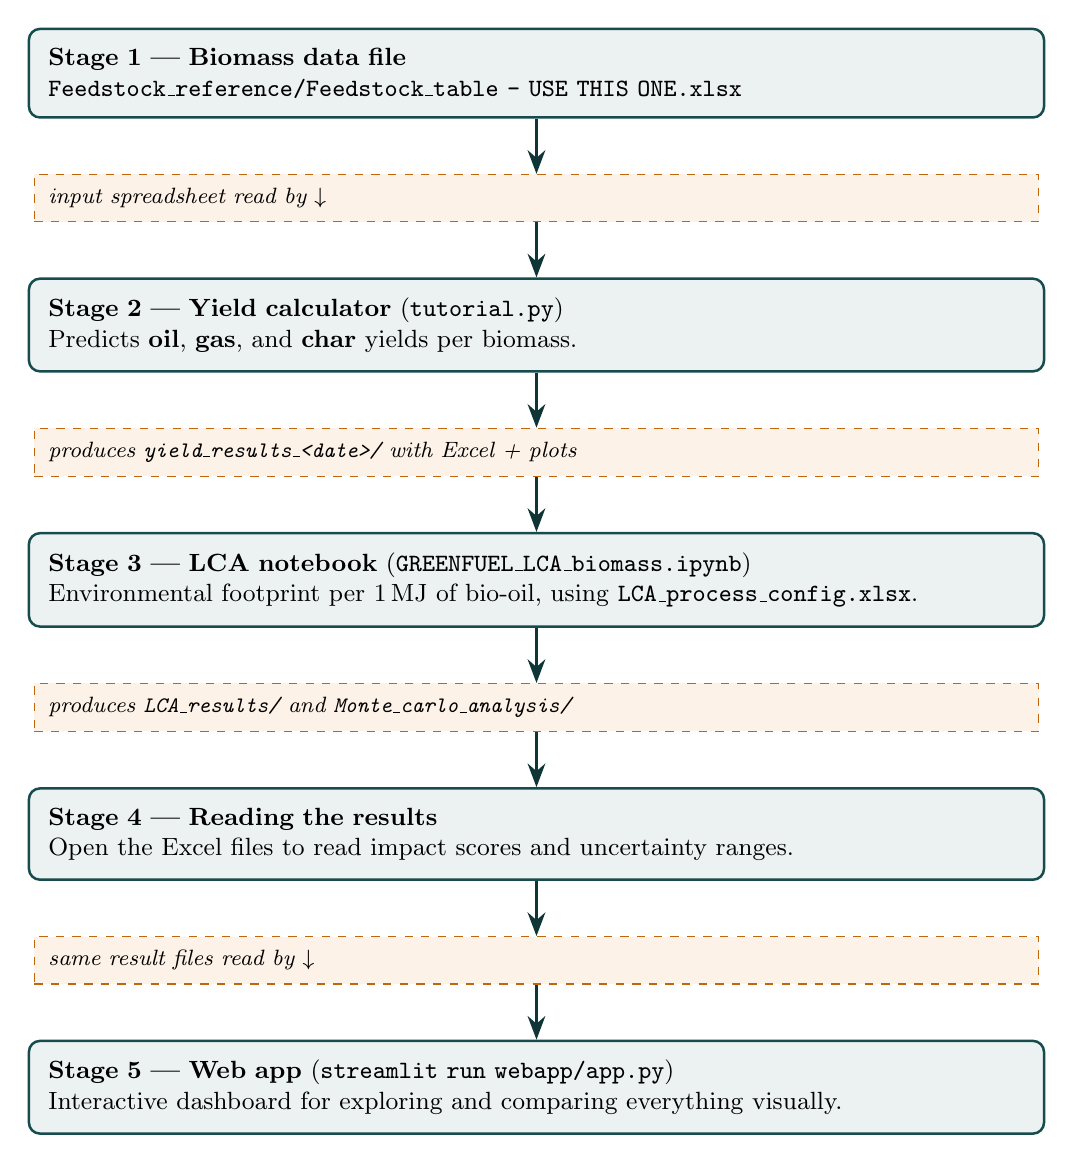
\begin{tikzpicture}[
  node distance = 7mm,
  stage/.style = {rectangle, rounded corners, draw=teal, line width=0.9pt,
                  fill=teal!8, text width=12.4cm, align=left, inner sep=7pt,
                  font=\small},
  file/.style  = {rectangle, draw=amber!85!black, dashed, fill=amber!10,
                  text width=12.4cm, align=left, inner sep=5pt,
                  font=\footnotesize\itshape},
  arr/.style   = {-{Stealth[length=3mm]}, line width=1pt, teal!70!black},
]
\node[stage] (s1) {\textbf{Stage 1 — Biomass data file}\\
  \texttt{Feedstock\_reference/Feedstock\_table - USE THIS ONE.xlsx}};
\node[file, below=of s1]  (f1) {input spreadsheet read by $\downarrow$};
\node[stage, below=of f1] (s2) {\textbf{Stage 2 — Yield calculator} (\texttt{tutorial.py})\\
  Predicts \textbf{oil}, \textbf{gas}, and \textbf{char} yields per biomass.};
\node[file, below=of s2]  (f2) {produces \texttt{yield\_results\_<date>/} with Excel + plots};
\node[stage, below=of f2] (s3) {\textbf{Stage 3 — LCA notebook} (\texttt{GREENFUEL\_LCA\_biomass.ipynb})\\
  Environmental footprint per 1\,MJ of bio-oil, using \texttt{LCA\_process\_config.xlsx}.};
\node[file, below=of s3]  (f3) {produces \texttt{LCA\_results/} and \texttt{Monte\_carlo\_analysis/}};
\node[stage, below=of f3] (s4) {\textbf{Stage 4 — Reading the results}\\
  Open the Excel files to read impact scores and uncertainty ranges.};
\node[file, below=of s4]  (f4) {same result files read by $\downarrow$};
\node[stage, below=of f4] (s5) {\textbf{Stage 5 — Web app} (\texttt{streamlit run webapp/app.py})\\
  Interactive dashboard for exploring and comparing everything visually.};
\draw[arr] (s1) -- (f1); \draw[arr] (f1) -- (s2);
\draw[arr] (s2) -- (f2); \draw[arr] (f2) -- (s3);
\draw[arr] (s3) -- (f3); \draw[arr] (f3) -- (s4);
\draw[arr] (s4) -- (f4); \draw[arr] (f4) -- (s5);
\end{tikzpicture}
\caption{The five stages and the files that connect them.}
\end{figure}

% =============================================================================
\section{Before You Start: Setup}
\label{sec:setup}
% =============================================================================

\subsection{System requirements}

\begin{itemize}
  \item \textbf{Operating system:} Windows 10/11, macOS 12+, or Linux
  \item \textbf{Python:} 3.10 or later (\href{https://www.python.org/downloads/}{python.org/downloads})
  \item \textbf{Disk space:} $\approx$500\,MB (including the virtual environment)
  \item \textbf{RAM:} 4\,GB minimum; 8\,GB recommended for full T/P sweeps
  \item \textbf{Browser:} any modern browser for the web application
\end{itemize}

\subsection{Environment A — \texttt{.venv} (Stages 1, 2, and 5)}

From inside the \code{BIOMASS\_to\_BIO-OIL} folder:

\begin{lstlisting}
python -m venv .venv
\end{lstlisting}

Activate it:

\begin{lstlisting}
# Windows (PowerShell)
.\.venv\Scripts\Activate.ps1

# macOS / Linux
source .venv/bin/activate
\end{lstlisting}

When active you will see \code{(.venv)} at the start of the prompt. Install dependencies (first time only):

\begin{lstlisting}
pip install -r requirements.txt
pip install -r webapp/requirements_webapp.txt
\end{lstlisting}

\notebox{PowerShell execution policy (Windows)}{If the activation command is blocked, run \texttt{Set-ExecutionPolicy -Scope CurrentUser RemoteSigned} in an elevated PowerShell, then try again.}

\subsection{Environment B — Brightway conda environment (Stage 3)}

The LCA notebook requires the Brightway~2.5 LCA framework in a separate conda
environment. Activate it with:

\begin{lstlisting}
conda activate bw25
\end{lstlisting}

The notebook also expects a Brightway \textbf{project} called
\code{GREENFUEL\_LCA\_WOOD} containing two databases:

\begin{itemize}
  \item \code{ecoinvent-3.12-cutoff} — background processes (electricity,
        transport, chemicals, \ldots)
  \item \code{ecoinvent-3.12-biosphere} — environmental flows (emissions,
        resource use)
\end{itemize}

\notebox{One-time prerequisite}{Importing ecoinvent requires an ecoinvent licence. If the project and databases are already on your machine you are ready. Setup instructions are in \texttt{LCA\_PROJECT/Project biomass/Setup.md}.}

% =============================================================================
\section{Stage 1 — The Biomass Data File}
% =============================================================================

Everything starts from one Excel workbook. The active copy is:

\begin{lstlisting}
BIOMASS_to_BIO-OIL/Feedstock_reference/Feedstock_table - USE THIS ONE.xlsx
\end{lstlisting}

\subsection{Sheet 1: \texttt{w.proximate+ultimate}}

One row per biomass type. Two standard laboratory analyses:

\begin{itemize}
  \item \textbf{Proximate analysis} (as-received): \code{M} = moisture, \code{VM} = volatile matter, \code{FC} = fixed carbon, \code{Ash} = ash
  \item \textbf{Ultimate analysis} (dry ash-free): elements \code{C}, \code{H}, \code{O}, \code{N}, \code{S} as weight percentages
\end{itemize}

\begin{table}[H]
\centering\small
\caption{Key columns in \texttt{w.proximate+ultimate}.}
\begin{tabular}{@{}lL{4.3cm}L{6.3cm}@{}}
\toprule
\textbf{Column} & \textbf{Meaning} & \textbf{Note} \\
\midrule
Feedstock Category    & broad group          & e.g.\ Wood, Agricultural wastes \\
Feedstock Subcategory & specific biomass     & e.g.\ ``Oak wood 1'' \\
M                     & moisture \%          & how wet the biomass is \\
VM                    & volatile matter \%   & the part that turns to gas/oil when heated \\
FC                    & fixed carbon \%      & solid carbon residue \\
Ash                   & ash \%               & inert mineral matter \\
C, H, O, N, S         & element \%           & N and S default to 0 if blank \\
\bottomrule
\end{tabular}
\end{table}

\subsection{Sheet 2: \texttt{bio-oil values}}

Describes the bio-oil produced from each biomass category: elemental composition
(\code{C}, \code{H}, \code{O}, \code{N}, \code{S}, \code{M}, \code{Ash}) and
energy content (\code{LHV}, \code{HHV} in MJ/kg).

\subsection{Data-entry tips}

The parser cleans the spreadsheet automatically:

\begin{itemize}
  \item \textbf{Comma decimals} like \code{10,5} are read as \code{10.5}
  \item \textbf{Ranges} like \code{10-20} are replaced by the midpoint \code{15}
  \item \textbf{Blank N or S} are treated as \code{0}
\end{itemize}

\notebox{Excel lock trap}{Do not leave the workbook open in Excel while running the calculator — it may be read-locked.}

% =============================================================================
\section{Stage 2 — Calculating Bio-oil Yields}
% =============================================================================

\subsection{Step 1: choose which workbook to read}
\label{sec:pickpath}

Open \code{tutorial\_workbook\_paths.py} and confirm the path:

\begin{lstlisting}[language=python]
WORKBOOK_PATHS = {
    "path1": "Feedstock_reference/Feedstock_table - USE THIS ONE.xlsx",
}
ACTIVE_WORKBOOK_PATH_KEY = "path1"
\end{lstlisting}

Add further entries (\code{"path2"}, \code{"path3"}) if you want to switch between workbooks without editing the path each time.

\subsection{Step 2: run the calculator}

With \code{.venv} active, from the \code{BIOMASS\_to\_BIO-OIL} folder:

\begin{lstlisting}
python tutorial.py
\end{lstlisting}

A full sweep over all feedstocks at the default temperature range (300--700\,°C) takes approximately 2--5 minutes.

\subsection{What the calculator does}

The model predicts the products of \textbf{fast pyrolysis} — heating biomass quickly without oxygen — using thermodynamic equilibrium: the mixture with the lowest total Gibbs free energy.

\paragraph{1. Reactive mass.} For 1\,kg as-received biomass:
\begin{equation}
m_{\text{dry}} = 1 - \frac{M}{100}, \qquad
m_{\text{reactive}} = m_{\text{dry}}\!\left(1 - \frac{\text{Ash}}{100}\right)
\end{equation}

\paragraph{2. Element moles.}
\begin{equation}
n_e = \frac{1000\,m_{\text{reactive}}\,(w_e/100)}{MW_e}, \qquad e \in \{C,H,O,N,S\}
\end{equation}

\paragraph{3. Heating values.} Channiwala--Parikh HHV correlation:
\begin{equation}
\text{HHV} = 0.3491C + 1.1783H + 0.1005S - 0.1034O - 0.0151N - 0.0211\text{Ash}
\end{equation}
\begin{equation}
\text{LHV} = \text{HHV} - 2.26\!\left(\tfrac{9H}{100} + \tfrac{M}{100}\right)
\end{equation}

\paragraph{4. Gibbs minimisation.} Find product amounts $n_i$ minimising total free energy:
\begin{equation}
\min_{\,n_i \ge 0} G_{\text{total}} = \sum_i n_i\mu_i, \qquad
\mu_i = g_i^0(T) + RT\ln\!\left(y_i\frac{P}{P^0}\right)
\end{equation}
subject to element conservation:
\begin{equation}
\sum_i a_{j,i}\,n_i = b_j \qquad j \in \{C,H,O,N,S\}
\end{equation}

\paragraph{5. Yields.}
\begin{equation}
Y_{\text{oil}} = \!\!\sum_{i\,\in\,\text{liquid}}\!\! n_i\frac{MW_i}{1000}, \qquad
Y_{\text{dry}} = \frac{Y_{\text{ar}}}{f_{\text{dry}}}, \qquad
Y_{\text{daf}} = \frac{Y_{\text{ar}}}{f_{\text{daf}}}
\end{equation}

\subsection{Output folder}

A timestamped folder is created, e.g.\ \code{yield\_results\_20260625\_094940/}:

\begin{table}[H]
\centering\small
\caption{Key contents of the output folder.}
\begin{tabular}{@{}lL{9cm}@{}}
\toprule
\textbf{File} & \textbf{Contents} \\
\midrule
\code{yield\_results.xlsx}       & full results: every feedstock × every T/P condition \\
\code{yield\_results\_clean.xlsx} & peak-yield summary \\
\code{van\_krevelen.png}         & H/C vs O/C composition plot \\
\code{ternary\_cho.png}          & barycentric C/H/O diagram \\
\code{peak\_yield\_vs\_temperature.png} & peak oil yield across temperature sweep \\
\bottomrule
\end{tabular}
\end{table}

Inside \code{yield\_results.xlsx} the most useful sheets are \code{results},
\code{acceptance\_summary}, \code{unmatched\_mappings}, \code{parse\_warnings},
and \code{solver\_warnings}.

\notebox{Yield basis}{``As-received (ar)'' includes moisture and ash. ``Dry'' removes moisture. ``Dry ash-free (daf)'' removes both. Always note which basis a yield refers to.}

% =============================================================================
\section{Stage 3 — Running the LCA Notebook}
% =============================================================================

\begin{lstlisting}
LCA_PROJECT/Project biomass/GREENFUEL_LCA_biomass.ipynb
\end{lstlisting}

\subsection{Launching the notebook}

\begin{lstlisting}
conda activate bw25
cd "LCA_PROJECT/Project biomass"
jupyter notebook GREENFUEL_LCA_biomass.ipynb
\end{lstlisting}

Run cells top to bottom with \textbf{Shift+Enter}, or use \textbf{Run $\rightarrow$ Run All Cells}.

\subsection{The USER CONFIG cell}

Near the top of the notebook is the only cell you normally edit:

\begin{table}[H]
\centering\small
\caption{Settings in the USER CONFIG cell.}
\begin{tabular}{@{}lL{8.8cm}@{}}
\toprule
\textbf{Setting} & \textbf{What it does} \\
\midrule
\code{BW\_PROJECT}    & Brightway project name (\code{'GREENFUEL\_LCA\_WOOD'}) \\
\code{ECOINVENT\_DB}  & background database (\code{'ecoinvent-3.12-cutoff'}) \\
\code{BIOSPHERE\_DB}  & environmental-flows database \\
\code{BIOMASS\_NAME}  & which biomass to analyse, e.g.\ \code{'Oak wood1'} \\
\code{d1, d2, d3}     & transport distances in km: feedstock→plant, oil→use, char→soil \\
\code{k\_el, k\_th}   & pyrolysis energy: electricity (kWh/kg) and heat (MJ/kg) \\
\code{MC\_ITERATIONS} & Monte~Carlo sample count (e.g.\ 10000) \\
\bottomrule
\end{tabular}
\end{table}

\notebox{Functional unit}{Every number is reported \textbf{per 1\,MJ of usable bio-oil}, allowing fair comparison between different biomass types and against fossil fuels.}

\subsection{What the notebook computes}

\paragraph{Reads Stage~2 results.} The notebook automatically finds the most recent \code{yield\_results\_*} folder and reads the yield, heating value, char, and gas quantities for your chosen biomass.

\paragraph{Scales to the functional unit.}
\begin{align}
z &= \frac{1}{\text{HHV}} & &\text{kg bio-oil per 1\,MJ}\\
y &= \frac{z}{Y_{\text{oil}}/100} & &\text{kg biomass needed}\\
\text{tkm} &= d \cdot \frac{\text{mass}}{1000} & &\text{transport work per leg}
\end{align}

\paragraph{Biogenic carbon accounting.} Two flows follow standard LCA practice for biomass:

\begin{itemize}
  \item \textbf{Combustion CO\textsubscript{2}} is logged as \code{Carbon dioxide, non-fossil} (GWP = 0), because the carbon originally came from the atmosphere.
  \item \textbf{Biochar carbon stored in soil} is logged as \code{Carbon dioxide, to soil or biomass stock} (factor = $-1$), a credit that can make the climate score \emph{negative}.
\end{itemize}

\paragraph{Impact calculation.} Uses the \textbf{ReCiPe 2016} method across 18 midpoint categories and 3 endpoint areas.

\paragraph{Monte~Carlo uncertainty.} Recalculates \code{MC\_ITERATIONS} times with randomly varied parameters to quantify sensitivity.

\subsection{Output files}

\begin{itemize}
  \item LCA scores: \code{LCA\_results/lca\_results\_<BIOMASS>.xlsx}
  \item Uncertainty: \code{Monte\_carlo\_analysis/montecarlo\_<BIOMASS>.xlsx}
\end{itemize}

% =============================================================================
\section{Stage 3b — Editing the LCI When Needed}
\label{sec:lci}
% =============================================================================

The Life-Cycle Inventory (LCI) — the ``recipe'' listing every input and emission — is edited in one Excel file without touching the notebook:

\begin{lstlisting}
LCA_PROJECT/Project biomass/LCA_process_config.xlsx
\end{lstlisting}

\begin{table}[H]
\centering\small
\caption{Sheets in \texttt{LCA\_process\_config.xlsx}.}
\begin{tabular}{@{}lL{9.3cm}@{}}
\toprule
\textbf{Sheet} & \textbf{Purpose} \\
\midrule
\code{Biomass\_Selection} & one row per biomass: yields, heating value, moisture, distances \\
\code{LCI\_Mapping}       & the recipe: each ingredient/emission and its ecoinvent process \\
\code{Parameters}         & reference list of all formula symbols (\code{y}, \code{z}, \code{k\_el}, \ldots) \\
\code{How\_To\_Use}       & built-in instructions \\
\bottomrule
\end{tabular}
\end{table}

Three typical edits:

\begin{enumerate}
  \item \textbf{Swap a background process} — find the relevant row in \code{LCI\_Mapping} and replace \code{ecoinvent\_process\_name} with the new process name.
  \item \textbf{Change an amount} — edit the \code{amount\_formula} cell using the symbols from \code{Parameters}.
  \item \textbf{Add a new biomass} — add a row in \code{Biomass\_Selection} with name, yields, heating value, moisture, and distances.
\end{enumerate}

\notebox{After editing}{Save and close the Excel file, then re-run the notebook (Run All Cells). It reads the file fresh each time.}

% =============================================================================
\section{Stage 4 — Reading the LCA Results}
% =============================================================================

Open the results file for your biomass:

\begin{lstlisting}
LCA_PROJECT/Project biomass/LCA_results/lca_results_<BIOMASS>.xlsx
\end{lstlisting}

\begin{table}[H]
\centering\small
\caption{Sheets in an \texttt{lca\_results\_*.xlsx} file.}
\begin{tabular}{@{}lL{9.3cm}@{}}
\toprule
\textbf{Sheet} & \textbf{What it shows} \\
\midrule
\code{All Categories} & all 18 ReCiPe midpoint impact categories \\
\code{Top 4}          & climate change plus the three biggest other impacts \\
\code{Endpoint}       & impacts rolled up into human health, ecosystems, and resources \\
\bottomrule
\end{tabular}
\end{table}

\begin{itemize}
  \item The \textbf{unit changes per category} — always read the unit column.
  \item Every score is \textbf{per 1\,MJ of bio-oil}.
  \item A \textbf{larger positive number is worse}; a \textbf{negative score} means a net environmental benefit.
\end{itemize}

\subsection{Why climate change can be negative}
\label{sec:negative}

A negative GWP score (e.g.\ $-0.029$\,kg CO\textsubscript{2}-eq) means the bio-oil is a net carbon sink for that step: carbon locked into biochar outweighs the fossil emissions from production and transport.

% =============================================================================
\section{Stage 4b — Reading the Monte~Carlo Uncertainty Results}
% =============================================================================

Results are in \code{LCA\_PROJECT/Project biomass/Monte\_carlo\_analysis/}.

\begin{table}[H]
\centering\small
\caption{Key columns in the \texttt{Summary} sheet of each Monte~Carlo file.}
\begin{tabular}{@{}lL{8.8cm}@{}}
\toprule
\textbf{Column} & \textbf{Meaning} \\
\midrule
\code{deterministic\_score} & single best estimate from Stage~4 \\
\code{mc\_mean}, \code{mc\_std} & mean and standard deviation across all samples \\
\code{cv\_pct} & coefficient of variation (spread as \% of mean) \\
\code{q1}, \code{median}, \code{q3} & 25th, 50th, 75th percentiles \\
\code{lower\_whisker}, \code{upper\_whisker} & typical range (box-plot fences) \\
\code{n\_iterations} & number of samples drawn \\
\bottomrule
\end{tabular}
\end{table}

A \textbf{low \code{cv\_pct}} (under 10\,\%) indicates a robust result; a
\textbf{high \code{cv\_pct}} (over 30\,\%) signals high sensitivity — treat
those scores with caution.

\notebox{Theoretical basis caveat}{The LCA is built on thermodynamic equilibrium yields, which represent an upper bound on what a real reactor can achieve. Real fast-pyrolysis reactors typically produce 60--80\,\% of the equilibrium bio-oil yield. This means the biomass input and energy consumption per MJ of bio-oil in the model are underestimated, and the true environmental burden per functional unit will be somewhat higher. Results should be interpreted as \emph{optimistic estimates} and compared against experimentally measured yields where possible.}

% =============================================================================
\section{Stage 5 — The Web App}
% =============================================================================

\begin{lstlisting}
cd BIOMASS_to_BIO-OIL
streamlit run webapp/app.py
\end{lstlisting}

A browser tab opens at \code{http://localhost:8501}. Use the \textbf{left sidebar} to switch pages. Press \code{Ctrl+C} in the terminal to stop.

\notebox{Where the app gets its data}{The app reads the latest \code{yield\_results\_*} folder, the \code{LCA\_results} folder, and the \code{Monte\_carlo\_analysis} folder. If a page looks empty, the corresponding earlier stage has not been run yet.}

\subsection{Home}

Welcome page explaining the model and its vocabulary. The sidebar lets you choose which results folder to use and toggle fast vs.\ full mode; it also reports how many biomass types loaded and how many calculations converged.

\screenshotslot{The Home page with the sidebar results-folder picker visible.}

\subsection{Explorer}

Browse all biomass types. Filter by category, yield basis, oil-yield range, and temperature; view a ranked bar or radial chart of oil yields. An expandable table shows detailed numbers, and a \textbf{Van Krevelen diagram} plots the H/C vs O/C chemical fingerprint of each biomass.

\screenshotslot{The Explorer page showing the oil-yield ranking and filters.}

\subsection{Comparison}

Put 2--8 biomass types side by side via a three-step sidebar (choose category, then specific biomasses, then yield basis). Two charts follow: the oil/gas/char split at each biomass's best condition, and how products change as temperature rises.

\screenshotslot{The Comparison page with several biomasses selected.}

\subsection{Environmental Impacts}

Shows Monte~Carlo uncertainty as Plotly box-and-whisker plots, one chart per impact category, for the biomasses you select. The box spans the interquartile range, the whiskers extend to 1.5$\times$IQR, and the single most extreme outlier on each side is shown as a dot. A \textbf{red diamond} marks the deterministic score. A legend in the top-right corner explains each symbol. An expandable table lists the summary statistics.

\screenshotslot{The Environmental Impacts page with box plots and red diamond markers.}

\subsection{Marine Transport}

A scenario explorer asking: \emph{how far could a cargo ship sail on each bio-oil compared with fossil heavy fuel oil?} Set the cargo, distance, and route (a China\,$\rightarrow$\,Denmark preset is included), pick a ``reach basis'' (equal carbon budget or equal feedstock energy), and the page draws a voyage illustration plus per-category impact bars with a dashed fossil-fuel reference line on the climate chart.

\screenshotslot{The Marine Transport page with the voyage illustration and impact bars.}

% =============================================================================
\section{Troubleshooting \& FAQ}
% =============================================================================

\begin{description}[leftmargin=0pt, style=nextline]
  \item[``Workbook not found'' when running \texttt{tutorial.py}.]
        Check \code{tutorial\_workbook\_paths.py}: the selected path must point to an existing \code{.xlsx} file that is not currently open in Excel.
  \item[No output folder was created.]
        The run stopped early. Read the terminal messages and confirm both required sheets and their columns are present in the workbook.
  \item[Many rows in \texttt{unmatched\_mappings}.]
        The feedstock subcategory name in \code{w.proximate+ultimate} column~B does not resemble any entry in \code{bio-oil values} column~B. Align the names or add a synonym.
  \item[The notebook cannot find a process or ``no ReCiPe methods''.]
        The Brightway project \code{GREENFUEL\_LCA\_WOOD} or its ecoinvent databases are not set up, or the process name in \code{LCI\_Mapping} is misspelled. See \texttt{LCA\_PROJECT/Project biomass/Setup.md}.
  \item[The notebook used old yields.]
        It always reads the \emph{most recent} \code{yield\_results\_*} folder. Re-run Stage~2 after updating the biomass data.
  \item[A web-app page is empty.]
        The required results files have not been generated. Run the corresponding earlier stage first.
  \item[Climate-change score is negative.]
        Expected, not a bug — see Section~\ref{sec:negative}.
\end{description}

% =============================================================================
\section{Running the Tests}
% =============================================================================

To verify your installation:

\begin{lstlisting}
cd BIOMASS_to_BIO-OIL
python -m unittest discover tests -v
\end{lstlisting}

All tests should pass on a clean installation.

% =============================================================================
\section*{Glossary}
\addcontentsline{toc}{section}{Glossary}
% =============================================================================

\begin{description}[leftmargin=0pt, style=nextline]
  \item[Pyrolysis] Heating biomass quickly \emph{without oxygen} so it decomposes into liquid (bio-oil), gas (syngas), and solid (char) instead of burning.
  \item[Bio-oil] The dark liquid fuel produced by pyrolysis.
  \item[Char / biochar] The carbon-rich solid residue; storing it in soil sequesters carbon.
  \item[Yield] The fraction of the biomass that becomes a given product, reported on as-received (ar), dry, or dry ash-free (daf) bases.
  \item[As-received / dry / daf] Three yield bases: counting the wet biomass, the dried biomass, or the dry and ash-free biomass respectively.
  \item[LCA (Life-Cycle Assessment)] A method for quantifying the total environmental impact of a product across its whole life.
  \item[LCI (Life-Cycle Inventory)] The detailed list of every input and emission in an LCA — the ``recipe''.
  \item[Functional unit] The fixed reference basis. Here: \textbf{1\,MJ of usable bio-oil}.
  \item[Brightway / ecoinvent] Brightway is the LCA software; ecoinvent is the background database of industrial processes it draws on.
  \item[ReCiPe 2016] The impact assessment method used to convert emissions into environmental scores (18 midpoints, 3 endpoints).
  \item[GWP (Global Warming Potential)] Climate-change impact, in kg CO\textsubscript{2}-equivalent per functional unit.
  \item[Midpoint / endpoint] Midpoints are specific environmental problems (climate, toxicity, land use, \ldots); endpoints group them into human health, ecosystem quality, and resource availability.
  \item[Monte~Carlo analysis] Recalculating many times with randomly varied inputs to quantify the uncertainty in a result.
  \item[Thermodynamic equilibrium yield] The maximum theoretically possible yield at a given temperature and pressure — an upper bound, not a guaranteed reactor outcome.
\end{description}

\end{document}
